%\usepackage{extsizes}
\documentclass[14pt, a4paper, russian]{report}

\linespread{1.3}

\usepackage{titlesec}
\usepackage[centertags]{amsmath}
\usepackage{amsthm,amsfonts,amssymb}
\usepackage{indentfirst}

\usepackage{extsizes}
\usepackage[left=25mm,right=10mm,top=20mm,bottom=20mm,bindingoffset=0cm]{geometry}

\usepackage{cmap}
\usepackage{multirow}
\usepackage{float}
\usepackage{mathtools}
\DeclarePairedDelimiter\ceil{\lceil}{\rceil}
\DeclarePairedDelimiter\floor{\lfloor}{\rfloor}

\usepackage{qtree}

\usepackage[T2A]{fontenc}
\usepackage[utf8]{inputenc}
\usepackage[english,russian]{babel}
%\usepackage{pscyr}
\RequirePackage{graphicx}
\RequirePackage{subfig}
\RequirePackage{pgfplots}
\usepackage{thmtools}   
\usepackage{hyperref}
\usepackage[nameinlink]{cleveref}
\usepackage{caption}


\newtheorem{lemma}{\indent Лемма}
\newtheorem{theorem}{\indent Теорема}
\newtheorem{corollary}{\indent Следствие}
\newtheorem{problem}{\indent Задача}
\newtheorem{remark}{\indent Замечание}
\newtheorem{definition}{\indent Определение}
\newtheorem{proposition}{\indent Утверждение}
\newtheorem{example}{\indent Пример}
\newtheorem{notation}{\indent Обозначение}

\crefname{lemma}{л.}{л.}
\crefname{theorem}{теор.}{теор.}
\crefname{corollary}{след.}{след.}
\crefname{definition}{опр.}{опр.}
\crefname{proposition}{утв.}{утв.}
\crefname{example}{прим.}{прим.}
\crefname{notation}{обозн.}{обозн.}
\crefname{remark}{замеч.}{замеч.}

\crefname{theorem}{Теорема}{Теорема}
\newcommand{\order}[2]{#1_{(#2)}}

\newcommand{\T}{^{\text{\tiny\sffamily\upshape\mdseries T}}}

\graphicspath{{./img/}}


\def\XYtext(#1,#2)#3{\rlap{\kern#1\lower-#2\hbox{#3}}}

% Переопределение вставки графики
\newcounter{PictureNo}

\hyphenpenalty 100
\tolerance 10000


\newenvironment{Proof}%
    {\par\noindent{\bf Доказательство.}}%
    {\hfill$\scriptstyle\blacksquare$}

\usepackage{bbm}
\bibliographystyle{unsrt}


\DeclareCaptionLabelSeparator{dash}{ –- }

\addto\captionsenglish{\renewcommand{\figurename}{Рисунок}}
\addto\captionsenglish{\renewcommand{\tablename}{Таблица}}
\addto\captionsenglish{\renewcommand{\bibname}{Список использованных источников}}
\captionsetup[figure]{labelfont=footnotesize,textfont=footnotesize,labelsep = dash}
\captionsetup[table]{labelfont=footnotesize,textfont=footnotesize,labelsep = dash}

\addto\captionsenglish{\renewcommand{\proofname}{Доказательство}}

\makeatletter % эта строка НЕОБХОДИМА!
\renewcommand{\@chapapp}{Глава} 
\addto\captionsenglish{% Replace "english" with the language you use
  \renewcommand{\contentsname}%
    {Оглавление}%
}

\titleformat{\chapter}[display]
{\normalfont\bfseries\center}
{Глава \thechapter. }{0em}{}

\titleformat{\section}[block]
{\normalfont\bfseries\center}
{\thesection. }{0em}{}

\titleformat{\subsection}[block]
{\normalfont\bfseries\center}
{\thesubsection. }{0em}{}

\newcommand\thefontsize[1]{{#1 The current font size is: \f@size pt\par}}

\begin{document}
\begin{center}
\hfill \break
\small{Федеральное государственное автономное образовательное учреждение \linebreak 
высшего образования}\\ 
\small{<<Московский физико-технический институт (государственный университет)>>}\\
\hfill \break
\small{Факультет инноваций и высоких технологий}\\
\small{Кафедра анализа данных}\\
\end{center}
\small{\textbf{Направление подготовки:} 01.03.02 Прикладная математика и информатика}\\
\hfill \break
\hfill \break
\hfill \break
\hfill \break
\begin{center}
\normalsize{\textbf{Автоматическая расстановка ударений в словах}}\\
\small{Бакалаврская работа}\\
\hfill \break
\hfill \break
\end{center}
 
\hfill \break
 
\begin{flushright}
\small{ 
\begin{tabular}{rl}
\textbf{Обучающийся:} & ФИО \\
 & \underline{\hspace{3cm}} \\\\
\textbf{Научный руководитель:} & должность\\
            & ФИО \\
 & \underline{\hspace{3cm}} \\\\
\end{tabular}
}
\end{flushright}

\hfill \break
\hfill \break
\hfill \break
\hfill \break
\begin{center} Москва 2018 \end{center}
\thispagestyle{empty} % выключаем отображение номера для этой страницы
 
% КОНЕЦ ТИТУЛЬНОГО ЛИСТА
 
\newpage
\begin{normalsize}
\chapter*{Аннотация}


Умные слова в 1500 знаков


\tableofcontents{}


\chapter*{Введение}
\addcontentsline{toc}{chapter}{Введение}
Ударение в словах – важнейший элемент устной, письменной и внутренней речи. В русском языке оно играет исключительно важную роль, так как благодаря ему мы можем различать слова. Одной из сложностей русского языка является его свободное ударение, которое не закреплено за каким-либо определенным слогом или морфемой слова. Любой слог может выделяться фонетически. К тому же ударение  может меняться с изменением грамматической формы слова. Как отмечает лингвист Н. А. Еськова, «слова с подвижным ударением в русском языке исчисляются сотнями. В процентном отношении это немного, но среди них много чрезвычайно употребительных, поэтому в речи они достаточно заметны» \cite{eskina}. Например: фл\'{а}г — фл\'{а}га — фл\'{а}ги; но вр\'{а}г — враг\'{а} — враг\'{и} 

Есть языки, где ударение  всегда на одном и том же слоге — такое ударение называют фиксированным. Например, во французском ударение всегда на последнем слоге, в польском — на предпоследнем, в чешском — на первом. В русском языке аналогичные правила весьма размыты, поэтому если человек не знает, как правильно ставить ударение в слове, то по одному только его внешнему облику сделать правильный выбор бывает сложно.  Нет общих правил ударения и в заимствованных для русского языка словах . Иногда оно меняет свое место по сравнению с ударением в языке-источнике: ноутб\'{у}к, скелет\'{о}н, футб\'{о}л, хокк\'{е}й. А иногда сохраняет: буль\'{о}н, гардер\'{о}б, жалюз\'{и}.
Расстановка ударений, как часть задачи предсказания произношения, - важная составляющая  приложений, таких как: автоматическое распознавание речи, синтез речи, транслитерация. Кроме того – это необходимо всем, изучающим русский язык.


\newpage

\chapter{Литературный обзор}

Работы по предсказанию постановки ударений в словах велись в двух направлениях. На основе лингвистических правил \cite{church, williams} и на основе анализа данных, где модели строятся напрямую из текстов с обозначенными ударениями. 

В русском языке сохраняется множество индо-европейских шаблонов ударений. Чтобы узнать ударение морфологически сложного слова, состоящего из основы и окончания, необходимо узнать является ли основа ударной и на какой слог падает в ней ударение, либо ударным является окончание \cite{halle}.
\section{Предсказание ударения в слове на основе ранжирования}
Авторы \cite{hall} рассмотрели проблему расстановки ударений, как задачу ранжирования. В своем исследовании  они опирались на более раннюю статью \cite{dou}. Из каждого слова выделяются гласные буквы и они предполагаются, как возможные варианты постановки ударений. Целью модели является отранжировать варианты так, чтобы верная гипотеза имела наименьший ранг.

Для ранжирования гипотез применялось Maximum Entropy ранжирование \cite{collins}. Во время обучения модели ей подавался набор правильных гипотез и их признаков. Во время предсказания в модель подавались все гипотезы, и в качестве верной выбиралась гипотеза с максимальным предсказанным результатом. В качестве основы для ранжирования использовалась линейная модель, вместо SVM, так как она более эффективна с вычислительной точки зрения для обучения и применения. 

В базовой статье \cite{dou} признаками являлись триграммы для гласных букв следующего вида: предыдущая согласная, если она есть, гласная буква, следующая за ней слогласная, если она есть (Dou). На основе лигвистического исследования в данной статье авторы добавили следующие признаки: для каждого слова взяты все начальные и конечные части (уже - у, уж, уже, е, же) (Affix). Также эти признаки добавлены в следующем виде: все буквы заменены на их абстрактные фонетические классы (представлены в \cref{table:phon_class})({Abstr Aff}).
\begin{table}[H]
		\caption{ Абстрактные фонетические классы}
	
	\begin{small}
		\begin{center}
			\begin{tabular}{|c|c|}
				\hline
				  Класс   &           Буквы            \\ \hline
				  vowel   & а, е, и, о , у, э, ю, я, ы \\ \hline
				  stop    &      б, д, г, п, т, к      \\ \hline
				  nasal   &            м, н            \\ \hline
				fricative &    ф, с, ш, щ, х, з, ж     \\ \hline
				hard/soft &            ъ, ь            \\ \hline
				   yo     &             ё              \\ \hline
				semivowel &            й, в            \\ \hline
				 liquid   &            р, л            \\ \hline
				affricate &            ц, ч            \\ \hline
			\end{tabular}
		\end{center}
	\end{small}
	\label{table:phon_class}
\end{table}

В качетсве данных авторы использовали Грамматический словарь русского языка Зализняка\cite{zaliz}, разбитый на обучающую и тестовую выборки. Из тестовой выборки также были отдельно выделены те слова, которые не встречались в обучающей выборке,  и для них также были получены  результаты. Результаты экспериментов представлены в \cref{table:range_res}.
\begin{table}[H]
		\caption{Результаты ранжирования}

	\begin{small}
		\begin{center}
			\begin{tabular}{|c|c|}
				\hline
				       Признаки         &             Accuracy score             \\ \hline
				\multicolumn{2}{|c|}{Тестовая выборка}                           \\ \hline
				          Dou           &                 0.972                  \\ \hline
				          Aff           &                 0.987                  \\ \hline
				     Aff+Abstr Aff      &                 0.987                  \\ \hline
				     Dou et al+Aff      &                 0.987                  \\ \hline
				Dou et al+Aff+Abstr Aff &                 0.987                  \\ \hline
				\multicolumn{2}{|c|}{Слова не встречавшиеся в обучающей выборке} \\ \hline
				          Dou           &                 0.806                  \\ \hline
				          Aff           &                 0.798                  \\ \hline
				     Aff+Abstr Aff      &                 0.810                  \\ \hline
				     Dou et al+Aff      &                 0.823                  \\ \hline
				Dou et al+Aff+Abstr Aff &                  0.89                  \\ \hline
			\end{tabular}
		\end{center}
	\end{small}
	\label{table:range_res}
\end{table}

Таблица показывает  влияние взаимодействия признаков на обобщающую способность модели, и лучший результат достигнут при использовании всех признаков.

Недостатками этой статьи является не использование контекста для определения места ударения. При подсчете результатов никак не учитывалась частота употребления слов в текстах языка, использовался просто его лексический набор.

\section{Предсказание ударения в слове при помощи конечного преобразователя}

Целью авторов\cite{reynolds} было разработки модели, которая могла быть помочь людям изучать русский язык, они решили что в некоторых словах ударение может быть пропущено. Авторы считали, что неправильное ударение может быть хуже, чем его отсутствие для человека осваиваюющего новый язык.

Модель состояла из двух частей: конечного преобразователя \cite{koskenniemi, karttunen}, который из полученного слова генерировал все возможные, корректные по его мнению, позиции ударения. Далее при помощи формальной грамматики \cite{karlsson} удалялись варианты, которые не подходили по контексту. Если после применения этой процедуры оставался один вариант прочтения, то он и выбирался как финальный. Если ни одного -- то ударение в слове не проставлялось. Если же вариантов было несколько -- то в зависимости от эксперимента выбиралась дальнейшая стратегия. 

Авторами использовался корпус текстов, состоящий из 7689 слов с размеченными ударениями, это были тексты для начинающих изучать русский язык. Также для обучения модели применялся Грамматический словарь русского языка Зализняка \cite{zaliz}. 

Описание экспериментов:
\begin{itemize}
	\item \textbf{bare:} при нескольких возможных вариантах прочтения  слова, ударение в слове не проставлялось.
	\item \textbf{safe:}  при нескольких возможных вариантах прочтения, ударение в слове выставлялось, если во всех них ударение падало на один и тот же слог.
	\item \textbf{randReading:} при нескольких возможных прочтениях, случайно выбиралось одно с вероятностью выбора варианта равной частоте встречаемости этого варианта в тексте.
	
	\item \textbf{freqReading:} при нескольких возможных прочтениях, выбирается вариант с максимальной  частотой встречаемости среди всех  вариантов в тексте.
\end{itemize}


Эксперименты были проведены при использовании формальной грамматики с учетом контекста и без него. Результаты представлены в \cref{table:final_state_result}. Для слов, которые не встретились в словаре, применялось простое правило постановки ударения: ударение падает на последню гласную, после которой идет согласная. Это является наиболее вероятным вариантом ударения в русском языке \cite{lavitskaya}. В результатх это отображено как guessSyl.

\begin{table}[H]
	\caption{Результаты применения конечного преобразователя}
	
	\begin{small}
		\begin{center}
			\begin{tabular}{|c|c|c|c|}
				\hline
				     Эксперимент      & Accuracy score & Доля ошибок & Доля пропущенных слов \\ \hline
				\multicolumn{4}{|c|}{Без грамматики}                                         \\ \hline
				        bare          &     30.43      &    0.17     &         69.39         \\ \hline
				        safe          &     90.07      &    0.49     &         9.44          \\ \hline
				     randReading      &     94.34      &    3.36     &         2.30          \\ \hline
				     freqReading      &     95.53      &    2.59     &         1.88          \\ \hline
				randReading+guessSyll &     94.99      &    4.05     &         0.96          \\ \hline
				freqReading+guessSyll &     95.83      &    3.46     &         0.72          \\ \hline
				\multicolumn{4}{|c|}{С грамматикой}                                          \\ \hline
				        bare          &     45.78      &    0.44     &         53.78         \\ \hline
				        safe          &     93.21      &    0.74     &         6.058         \\ \hline
				     randReading      &     95.50      &    2.59     &         1.90          \\ \hline
				     freqReading      &     95.73      &    2.40     &         1.88          \\ \hline
				randReading+guessSyll &     95.92      &    3.33     &         0.74          \\ \hline
				freqReading+guessSyll &     96.15      &    3.14     &         0.72          \\ \hline
			\end{tabular}
		\end{center}
	\end{small}
	\label{table:final_state_result}
	
\end{table}

При использовании модели без формальной грамматики полнота гипотез составила 97.55\%, что является максимумом результата для данной модели. При использовании грамматики полнота составила 97.35\%. Эти результаты являются потолком для соответствующих экспериментов. Совмещение всех моделей и предсказываение методом FreqReading  позволило получить наибольших процент правильных ударений. Метод расстановки ударений для неизвестных слов в данном случае имеет точность всего 21\%. При этом высокая точность была достигнута за счет расстановки ударений почти во всех словах, что соответственно повысило уровень ошибок. 

Метод, представленный в этой статье, является попыткой улучшить словарный метод, путем разрешения неоднозначностей в омографах при помощи формальной грамматики. При этом для слов, которые не  встретились в словаре работает очень простой и слабый алгоритм. В этом случае качество получается очень низким. Недостатком является также использование небольшого закрытого корпуса текстов. А так как использовались тексты для начинающих изучать язык, их словарь скорее всего был достаточно мал. Не ясна цель проведения эксперимента RandReading, так как несложно показать строго математически, что метод FreqReading всегда дает большую вероятность правильного ответа.

\section{Предсказание ударения в слове при помощи символьной нейронной сети}
\label{global_desc}
	В качестве основы для модели авторы \cite{ponomareva} использовалась  символьная двусторонняя рекуррентная нейронная сеть на основе LSTM-модулей. На вход подавалась матрица размера [длина фразы; число возможных символов]. Для кодирования символов было применено one-hot кодирование. Авторами выбрана следующая архитектура: к входной матрице применяется двусторонняя рекуррентная нейронная сеть, сконкатенированные вектора, полученные от рекуррентного слоя подаются в полносвязные слой с softmax активацией. На выходе получается вектор размера равного длине фразы, соответствующий распределению вероятностей постановки ударения в конкретной позиции.(представлена на \cref{fig:base_global})

\begin{figure}[H]
	\begin{center}
		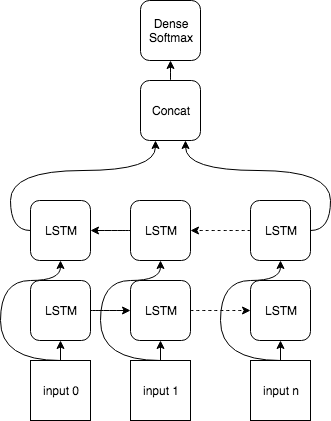
\includegraphics[width=0.5\linewidth]{Baseline}
	\end{center}
	\caption{\small{Архитектура сети}}
	\label{fig:base_global}
\end{figure}

Для разных экспериментов использовался грамматический словарь русского языка Зализняка \cite{zaliz} и база данных акцентологической разметки в составе национального корпуса русского языка \cite{grishina}. 

Авторами были проведены следующие эксперименты
\begin{enumerate}
	\item \textbf{Обучение и предсказание на основе словаря.} Словарь Зализняка был разделен на обучающую и тестовую выборки в соотношении 2:1. Результаты этого эксперимента представлены в \cref{table:dict_res}.
	\item \textbf{Обучение и предсказание на основе акцентологического корпуса.} С корпусом было проведено два эксперимента, в первом в качестве фразы использовалось только само слово. Во втором же, к нему были дописаны три последние буквы из слова, которое идет перед ним в предложении, если такое было. Сравнительные результаты экспериментов представлены в \cref{table:base_text}. Основная разница между моделями с контекстом и без него может быть видна только на омографах. Результаты применения на них представлены в \cref{table:base_homo}. Как видно из результатов модель успешно использует контекст для расстовки ударения в омографах во многих случаях.
\end{enumerate}

\begin{table}[H]
		\caption{Результаты применения нейросетевой модели на словаре Зализняка}
	
	\begin{small}
		\begin{center}
			\begin{tabular}{|c|c|c|c|}
				\hline
				    Экспериимент      & Accuracy score & Доля Ошибок & Доля пропущенных слов \\ \hline
				\multicolumn{4}{|c|}{Без грамматики}                                         \\ \hline
				        bare          &     30.43      &    0.17     &         69.39         \\ \hline
				        safe          &     90.07      &    0.49     &         9.44          \\ \hline
				     randReading      &     94.34      &    3.36     &         2.30          \\ \hline
				     freqReading      &     95.53      &    2.59     &         1.88          \\ \hline
				randReading+guessSyll &     94.99      &    4.05     &         0.96          \\ \hline
				freqReading+guessSyll &     95.83      &    3.46     &         0.72          \\ \hline
				\multicolumn{4}{|c|}{С грамматикой}                                          \\ \hline
				        bare          &     45.78      &    0.44     &         53.78         \\ \hline
				        safe          &     93.21      &    0.74     &         6.058         \\ \hline
				     randReading      &     95.50      &    2.59     &         1.90          \\ \hline
				     freqReading      &     95.73      &    2.40     &         1.88          \\ \hline
				randReading+guessSyll &     95.92      &    3.33     &         0.74          \\ \hline
				freqReading+guessSyll &     96.15      &    3.14     &         0.72          \\ \hline
			\end{tabular}
		\end{center}
	\end{small}
	\label{table:dict_res}
\end{table}

\begin{table}[H]
		\caption{Результаты применения нейросетевой модели на словаре Зализняка}
	
	\begin{small}
		\begin{center}
			\begin{tabular}{|c|c|c|c|}
				\hline
				    Экспериимент      & Accuracy score & Доля Ошибок & Доля пропущенных слов \\ \hline
				\multicolumn{4}{|c|}{Без грамматики}                                         \\ \hline
				        bare          &     30.43      &    0.17     &         69.39         \\ \hline
				        safe          &     90.07      &    0.49     &         9.44          \\ \hline
				     randReading      &     94.34      &    3.36     &         2.30          \\ \hline
				     freqReading      &     95.53      &    2.59     &         1.88          \\ \hline
				randReading+guessSyll &     94.99      &    4.05     &         0.96          \\ \hline
				freqReading+guessSyll &     95.83      &    3.46     &         0.72          \\ \hline
				\multicolumn{4}{|c|}{С грамматикой}                                          \\ \hline
				        bare          &     45.78      &    0.44     &         53.78         \\ \hline
				        safe          &     93.21      &    0.74     &         6.058         \\ \hline
				     randReading      &     95.50      &    2.59     &         1.90          \\ \hline
				     freqReading      &     95.73      &    2.40     &         1.88          \\ \hline
				randReading+guessSyll &     95.92      &    3.33     &         0.74          \\ \hline
				freqReading+guessSyll &     96.15      &    3.14     &         0.72          \\ \hline
			\end{tabular}
		\end{center}
	\end{small}
	\label{table:base_text}
\end{table}

\begin{table}[H]
		\caption{Результаты применения нейросетевой модели на омографах}
	
	\begin{small}
		\begin{center}
			\begin{tabular}{|c|c|c|c|}
				\hline
				    Экспериимент      & Accuracy score & Доля Ошибок & Доля пропущенных слов \\ \hline
				\multicolumn{4}{|c|}{Без грамматики}                                         \\ \hline
				        bare          &     30.43      &    0.17     &         69.39         \\ \hline
				        safe          &     90.07      &    0.49     &         9.44          \\ \hline
				     randReading      &     94.34      &    3.36     &         2.30          \\ \hline
				     freqReading      &     95.53      &    2.59     &         1.88          \\ \hline
				randReading+guessSyll &     94.99      &    4.05     &         0.96          \\ \hline
				freqReading+guessSyll &     95.83      &    3.46     &         0.72          \\ \hline
				\multicolumn{4}{|c|}{С грамматикой}                                          \\ \hline
				        bare          &     45.78      &    0.44     &         53.78         \\ \hline
				        safe          &     93.21      &    0.74     &         6.058         \\ \hline
				     randReading      &     95.50      &    2.59     &         1.90          \\ \hline
				     freqReading      &     95.73      &    2.40     &         1.88          \\ \hline
				randReading+guessSyll &     95.92      &    3.33     &         0.74          \\ \hline
				freqReading+guessSyll &     96.15      &    3.14     &         0.72          \\ \hline
			\end{tabular}
		\end{center}
	\end{small}
	\label{table:base_homo}
\end{table}

Как видно нейросетевая модель успешно справляется с использование контекста для расстановки ударений в омографах. Недостатками же представленной модели является очень простая архитектура и отсутствие работы с текстом. Далее мы будем использовать эту модель как базовую для сравнения результатов. 


\newpage
\chapter{Экспериментальная часть}
\section{Используемы данные}
\label{prepare}
Во всех экспериментах в качестве данных мы использовали база данных акцентологической разметки в составе национального корпуса русского языка \cite{grishina}. С каждым предложением в тексте были произведены следуюющие преобразование
\begin{enumerate}
	\item Все буквы приведены к строчным.
	\item Предложение разбито на смысловые подпредложение, используя в качестве разделителей знаки препинания. На этом этапе все знакия препинания удаляются.
	\item Подпредложение содержавшие символы кроме кириллических букв удалены.
	\item По правилам эксперимента из получившихся подпреложений собирались фразы.
\end{enumerate}
Итоговые данные состояли из 3285455  слов. Все данные были разделены на 3 части: обучающая выборка (2299818 слов), валидационная выборка, применяемая для подбора параметров во время обучения модели (49281 слов) и тестовую  выборку, на которые измерялся конечный результат (936356 слов).
Омографы среди всех слов в нашей выборке составляют 3.31\%. Распределение долей слов по длинам представлено в \cref{table:length_gen}. Аналогичное распределение для омографов представлено в \cref{table:length_homo}.

\begin{table}[H]
	\caption{Распределение слов по числу слогов}
	
	\begin{small}
		\begin{center}
			\begin{tabular}{|c|c|}
				\hline
				Число слогов & Доля слов \\ \hline
				     2       &   0.474   \\ \hline
				     3       &   0.308   \\ \hline
				     4       &   0.144   \\ \hline
				     5       &   0.053   \\ \hline
				     6       &   0.015   \\ \hline
				     7       &   0.003   \\ \hline
				     8       &   0.001   \\ \hline
				     9       & $10^{-4}$ \\ \hline
			\end{tabular}
			\end{center}
		\end{small}
	\label{table:length_gen}
\end{table}	
\begin{table}[H]
	\caption{Распределение омографов по числу слогов}
	
	\begin{small}
		\begin{center}
			\begin{tabular}{|c|c|}
				\hline
				Число слогов & Доля слов \\ \hline
				     2       &   0.736   \\ \hline
				     3       &   0.212   \\ \hline
				     4       &   0.051   \\ \hline
			\end{tabular}
		\end{center}
	\end{small}
	\label{table:length_homo}
\end{table}	



\section{Метрики}
Основной метрикой используемой для оценки окончательного качества является \textit{Accuracy score}  (\ref{eq:acc}). 

Обозначим позицию ударения во фразе как $y_i$. Позицию ударения, предсказанную моделью обозначим как $y^*_i$. Число фраз в выборке обозначим как $N$

\begin{align}
\label{eq:acc} ACC &= \frac{\sum\limits_{i=1}^{N}I \left\{y_i = y^*_i\right\}}{N} 
\end{align}

\section{Локальная модель}
В качестве самой простой нейросетевой архетектуры нами была выбрана данная. 
\subsection{Архитектура модели}
К входным данным применяется двустронняя рекурентная нейронная сеть на основе LSTM-модулей. Далее к каждому промежуточному вектору применяется один и тот же полносвязный слой с softmax активацией с размерностью выхода 2, первую компоненту этого вектора мы интерпретируем, как вероятность того что в данной позиции нет ударения, в вторую, как то что оно есть. Архитеткура представлена на \cref{fig:local}. Эту архитектуру далее мы будем называть локальной моделью. 

\begin{figure}[H]
	\begin{center}
		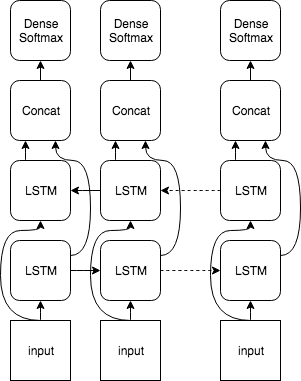
\includegraphics[width=0.5\linewidth]{Local}
	\end{center}
	\caption{\small{Архитектура сети}}
	\label{fig:local}
\end{figure}


\subsection{Посимвольный эксперимент}
Для получение более подробной картины того, как разные архитектуры нейронной сети и предобработка данных влияет на качество мы провели данный эксперимент, как упрощение базовой модели \cite{ponomareva}, которую мы будем называть глобальной моделью .

\textbf{Входные данные:} На вход модели подается слово, в котором мы хотим поставить ударение, 4 последние буквы предыдущего слова, если оно есть и 4 последние буквы следующего слова, если оно есть. 4 буквы мы используем, потому что это  длина  окончания в русском языке. Окончание может нам помочь определить форму слова, что необходимо для удаления неоднозначности при расстановки ударения в большинстве омографов.

Позиция ударения во фразе выбиралась, как позиция с максимальной вероятностью второго класса.

Результаты этого эксперимента и сравнение с базовой моделью представлены в \cref{table:local_char}

\begin{table}[H]
		\caption{Сравнение результатов локальной и глобальной символьной модели}
	
	\begin{small}
		\begin{center}
			\begin{tabular}{|c|c|c|}
				\hline
				Число слогов & Локальная модель & Глобальная модель \\ \hline
				\multicolumn{3}{|c|}{Все слова}                     \\ \hline
				     2       &      0.961       &       0.983       \\ \hline
				     3       &      0.940       &       0.977       \\ \hline
				     4       &      0.947       &       0.976       \\ \hline
				     5       &      0.960       &       0.977       \\ \hline
				     6       &      0.958       &       0.973       \\ \hline
				     7       &      0.924       &       0.955       \\ \hline
				     8       &      0.866       &       0.923       \\ \hline
				     9       &      0.809       &       0.952       \\ \hline
				  среднее    &      0.952       &       0.979       \\ \hline
				\multicolumn{3}{|c|}{Омографы}                      \\ \hline
				     2       &      0.839       &       0.810       \\ \hline
				     3       &      0.774       &       0.844       \\ \hline
				     4       &      0.787       &       0.847       \\ \hline
				  среднее    &      0.821       &       0.819       \\ \hline
			\end{tabular}
		\end{center}
	\end{small}
	\label{table:local_char}
\end{table}	

Наше предположение о том, что эта модель более слабая, чем глобальная подтвердилось. При этом благодаря изменению использования контекста, результаты на омографах удалось улучшить

\subsection{Эксперимент с предложением}

Для исследования влияния длины контекста на качество расстановки ударений был проведен следующий эксперимент. Контекстом здесь является не окончания соседних слов, а все подпредложение (часть предложения между знаками препинаниия). Если введение в контекст других слов кроме соседних является тоже значимым, мы поймем это в этом эксперименте.

\textbf{Входные данные:} На вход модели подается подпредложение, описание построение находится в \cref{prepare}. При этом модель должна расставить ударения во всех словах в подпредложении.

Для получения итогового результата из вектора с вероятностями мы в каждом слове выбирали символ с наибольшей вероятностью того, что на него падает ударение. Это в отличие отсечения по границе позволяет добиться того, что в каждом слове находится ровно одно ударение.

Результаты этого эксперимента и их сравнение с локальной символьной моделью представлены в \cref{table:local_sent}

\begin{table}[H]
		\caption{Сравнение локальной символьной модели и локальной модели по предложениям}
	\begin{small}
		\begin{center}
			\begin{tabular}{|c|c|c|}
				\hline
				Число слогов & Символьная модель & Модель по предложениям \\ \hline
				\multicolumn{3}{|c|}{Все слова}                          \\ \hline
				     2       &      0.961       &         0.897          \\ \hline
				     3       &      0.940       &         0.891          \\ \hline
				     4       &      0.947       &         0.902          \\ \hline
				     5       &      0.960       &         0.927          \\ \hline
				     6       &      0.958       &         0.925          \\ \hline
				     7       &      0.924       &         0.898          \\ \hline
				     8       &      0.866       &         0.855          \\ \hline
				     9       &      0.809       &         0.647          \\ \hline
				  среднее    &      0.952       &         0.898          \\ \hline
				\multicolumn{3}{|c|}{Омографы}                           \\ \hline
				     2       &      0.839       &         0.831          \\ \hline
				     3       &      0.774       &         0.754          \\ \hline
				     4       &      0.787       &         0.775          \\ \hline
				  среднее    &      0.821       &         0.812          \\ \hline
			\end{tabular}
		\end{center}
	\end{small}

	\label{table:local_sent}
\end{table}

\subsection{Слоговая модель}
\label{syl_descr}
В русском языке ударение может падать только на гласные буквы. Модели приходилось также учитывать то, что на согласные буквы ударение падать не может. Из-за этого увеличивалась сложность модели, и количество информации, которое оно должна хранить. Также из-за этого увеличивалось время обучения.

Одним из вариантов решения этой проблемы является замена символьной модели на слоговую, то есть на вход модели будут подаваться закодированные слоги, а не символы.

Деление на слоги слов в русском языке однозначно установлено \cite{litnevskaya}, поэтому в преобразование данных будет детерменированно. 

После преобразования получилось 14083 слога.

\textbf{Входные данные:} Формат входных данных аналогичен формату, примененному в локальной символьной модели.

Результаты этого эксперимента, а также их сравнение с результатами локальной и глобальной сисвольной моделей представлены в \cref{table:local_syl}

\begin{table}[H]
		\caption{Сравнение результатов локальной и глобальной символьной модлелей с локальной слоговой моделью}
	
	\begin{small}
		\begin{center}
			\begin{tabular}{|c|c|c|c|}
				\hline
				Число слогов & Слоговая модель & Локальная модель & Глобальная модель \\ \hline
				\multicolumn{4}{|c|}{Все слова}                                       \\ \hline
				     2       &      0.985      &      0.961       & 0.983             \\ \hline
				     3       &      0.972      &      0.940       & 0.977             \\ \hline
				     4       &      0.972      &      0.947       & 0.976             \\ \hline
				     5       &      0.976      &      0.960       & 0.977             \\ \hline
				     6       &      0.977      &      0.958       & 0.973             \\ \hline
				     7       &      0.947      &      0.924       & 0.955             \\ \hline
				     8       &      0.899      &      0.866       & 0.923             \\ \hline
				     9       &      0.843      &      0.809       & 0.952             \\ \hline
				  среднее    &      0.978      &      0.952       & 0.979             \\ \hline
				  \multicolumn{4}{|c|}{Омографы}                                        \\ \hline
				  
				     2       &      0.889      &      0.839       & 0.810             \\ \hline
				     3       &      0.832      &      0.774       & 0.844             \\ \hline
				     4       &      0.843      &      0.787       & 0.847             \\ \hline
				  среднее    &      0.877      &      0.821       & 0.819             \\ \hline
			\end{tabular}
		\end{center}
	\end{small}
	\label{table:local_syl}
\end{table}

Применение слогового кодирования позволило без изменения архитектуры модели повысить качество расстановки ударений на 2.6\% для всех слов. Это позволило этой модели сравняться по качеству с глобальной символьной моделью. При этом качество расстоновки удаления в омографах у этой модели выше. Из этого всего можно сделать вывод, что обучение модели на слогах вместо символов может помочь повысить результат  без изменения архитектуры. Это можно объяснить тем, что модель учит векторные представления для слогов отдельно в embedding слое, а не пытается выучить подобные взаимосвязи в рекуррентном слое. Или  в слоге содержится больше информации, чем в одной букве.

\section{Глобальная модель}
\subsection{Архитектура модели}
Архитектура этой модели совпадает с архитектурой базовой модели. Подробна она описана в \cref{global_desc}. 
Схема архитектура представлена на \cref{fig:base_global2}

\begin{figure}[H]
	\begin{center}
		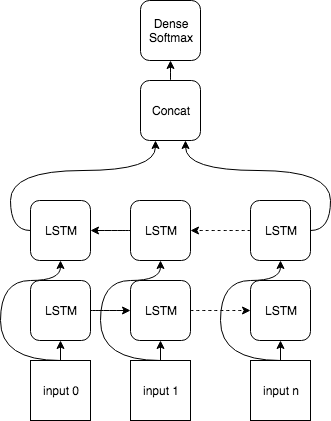
\includegraphics[width=0.5\linewidth]{Baseline}
	\end{center}
	\caption{\small{Архитектура сети}}
	\label{fig:base_global2}
\end{figure}

\subsection{Символьная модель}
Эта модель является нашей базовой. Опиисание данных и результаты этой модели представлены в выше в литературном обзоре в \cref{global_desc}

\subsection{Слоговая модель}
Использование слоговой, как базовой входной единицей модели показало положительный результат в при использовании с локальной моделью. Мы рассчитываем также положительного результата с глобальной моделью.

Результаты этого эксперимента, и их сравнение с  

\begin{table}[H]
	\caption{Сравнение результатов локальной и глобальной слоговой модлелей с глобальной символьной моделью}
	
	\begin{small}
		\begin{center}
			\begin{tabular}{|c | c | c|c|}
				\hline
				Число слогов & Глобальная модель & Локальная модель & Символьная модель \\ \hline
				\multicolumn{4}{|c|}{Все слова}                                       \\ \hline
				2       & 0.985  &      0.985      & 0.983             \\ \hline
				3       &   0.978 &      0.972      & 0.977             \\ \hline
				4       &   0.977 &      0.972      & 0.976             \\ \hline
				5       &  0.977 &      0.976      & 0.977             \\ \hline
				6       &  0.970 &      0.977      & 0.973             \\ \hline
				7       &  0.945 &      0.947      & 0.955             \\ \hline
				8       &  0.895 &      0.899      & 0.923             \\ \hline
				9       & 0.849 &      0.843      & 0.952             \\ \hline
				среднее    & 0.981 &      0.978      & 0.979             \\ \hline
				\multicolumn{4}{|c|}{Омографы}                                        \\ \hline
				
				2       & 0.893&      0.889      & 0.810             \\ \hline
				3       & 0.847&      0.832      & 0.844             \\ \hline
				4       & 0.852&      0.843      & 0.847             \\ \hline
				среднее    & 0.882 &      0.877      & 0.819             \\ \hline
			\end{tabular}
		\end{center}
	\end{small}
	\label{table:global_syl}
\end{table}
В глобальнной модели использование слогового кодирования также дало повышение результата по сравнению с символьной моделью. Поэтому далее символьные модели мы больше не будем рассматривать.  Также это первая модель, которая показала лучший результат, чем базовая модель. 

Глобальная модель  по сравнениию с локальной имеет большие проблемы с расстановкой ударения в слогах более чем из 7 слогов. Это можно объяснить тем, что такие слова очень редко встречаются и полносвязный слой выучивает, что последние слоги почти всегда безударные. Глобальной модели нужен гораздо более сильный сигнал, для постановки ударения в такую позицию по сравнению с локальной. В локальной же модели полносвязный слой применяется в каждой позиции независимо, поэтому зависимости от позиции менее выражена. В символьной модели этот эффект меньше проявлен, так как длина слова в слогах и буквах не связана линейно, поэтому более длинные слова там встречаются чаще. 

\section{Модель с attention слоем}
Значительного увеличения качества в машинном переводе удалось добится благодаря замене encoder-decoder архитектуры на основе только рекуррентного слоя добавление attention механизма. 
\subsection{Описание attention механизма}
Описание attention мехаизма производится на основе одной из первых статей, где он был представлен \cite{bahdanau}. Описанный далее attention механизм также известен как soft attention.

Целью attention-механизма является по вектору текущего состояния ($v_i$), векторам промежуточных состояний кодирующего слоя ($h_t, t \in [0; l)$, где $l$ - длина входных данных), чаще всего это слой на основе рекуррентных модулей предсказать вектор текущего состояния ($a_i$), который будет проинтерпретирован в соответствие с поставленной задачей. 
Сначала для каждого промежутного вектора вычисляется его значимость по отношение к текущему состоянию (\ref{eq:score}). Далее полученные значимости преобразуются в веса для каждой позиции  $\alpha_{i,t}$ при помощи sotmax преобразования (\ref{eq:prob}). Взвешенная сумма промежуточных векторов $h_t$ с весами $\alpha_{i,t}$ называется контекстным вектором $c_i$ \ref{eq:att_vec}. Выходной вектор получается из контекстного линейным преобразованием и затем покоординатным нелинейным преобразованием. В данном случае -- это гиперболический тангенс (\ref{eq:out_vector}).

\begin{align}
\label{eq:score} score(h_t, v_i) = v_i^Ttanh\left( W_1 v_i + W_2 h_t\right) \\
\label{eq:prob} \alpha_{i,t}=\frac{\exp\left(score\left(h_t,   v_i\right) \right) }{\sum\limits_{k=0} ^{l-1} \exp\left(score\left(h_k,   v_i\right) \right)}\\
\label{eq:att_vec} c_i = \sum\limits_{t=0}^{l-1} \alpha_t h_t \\
\label{eq:out_vector} a_i = tanh\left(W_3 c_i \right)  \\
\end{align}
 
В представленных выше уравнениях $W_i$ - матрицы линейных преобразований.

Благодаря подсчету весов в каждом промежуточном состоянии можно визуализировать то какие части входа были наиболее важными для получения результата в конкретно этой позиции. При использовании attention механизма в нейросетевом машинном переводе такая визуализация получается хорошо интерпретируемой: для перевода текущего слова наиболее важными являются оригинальные слово или слова, которые передают его смысл. Пример при переводе с французского языка на английский язык представлен на \cref{fig:att_map}

\begin{figure}[H]
	\begin{center}
		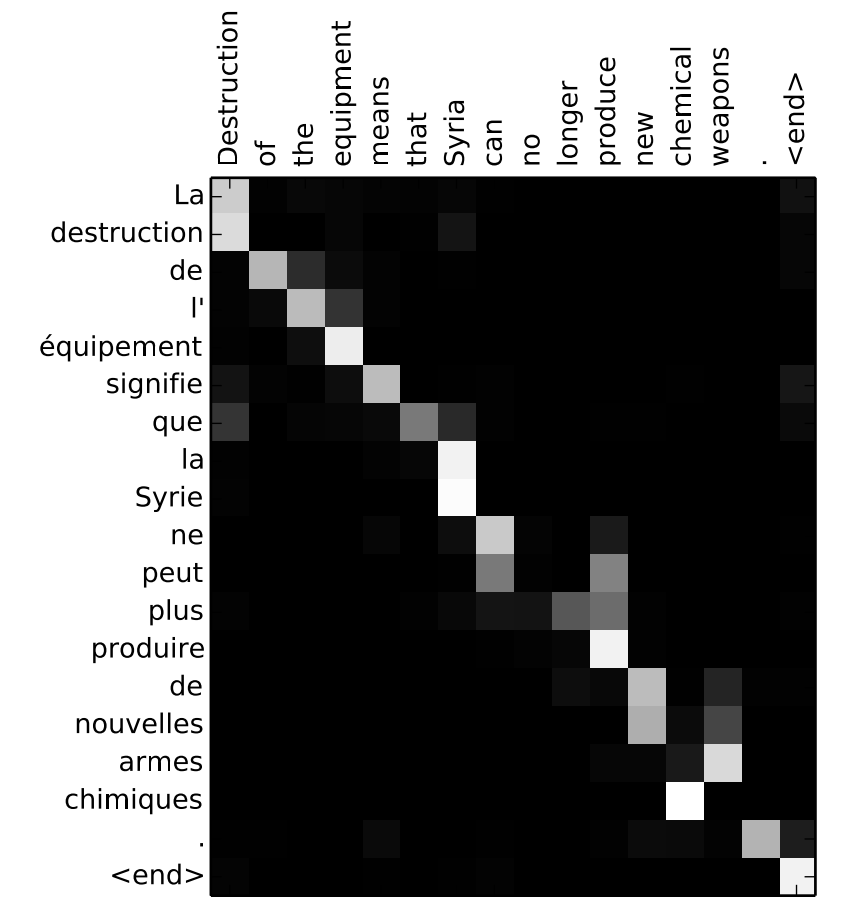
\includegraphics[width=0.5\linewidth]{AttentionMap}
	\end{center}
	\caption{\small{Визуализация весов $\alpha_{i,t}$ при переводе}}
	\label{fig:att_map}
\end{figure}


\subsection{Архитектура модели}
Так как нам нужно предсказать только вектор распределения вероятности ударения в конкретной позиции мы не будем использовать декодирующую сеть, а сразу однократным применением attention слоя получим искомый вектор.
Модель состоит из двустороннего рекуррентного слоя на основе LSTM модулей. К выходному вектору рекуррентного слоя применяется полносвязный слой, полученный вектор будет рассматривать как вектор текущего состояния для attention слоя. Далее следует attention слой и к полученному на его выходе вектору применяется полносвязный слой с softmax активацией.

Схема этой архитектуры представлена на \cref{fig:att}

\begin{figure}[H]
	\begin{center}
		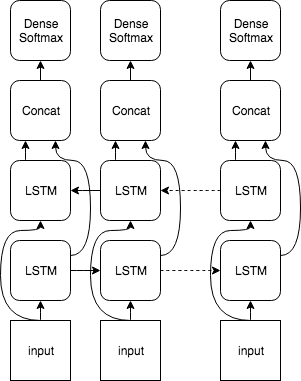
\includegraphics[width=0.5\linewidth]{Local}
	\end{center}
	\caption{\small{Архитектура сети с attention}}
	\label{fig:att}
\end{figure}


Для нашей модели примение attention механизма можно считать отчасти объединениием локального и глобального подхода: мы используем все промежуточные состояния рекуррентного слоя, как в локальной модели. При этом предсказываем сразу распределение вероятностей поставить ударение в конкретную позицию, как в глобальной модели.
\subsection{Слоговая модель}
\section{Эксперименты с BPE токенизацией}



\section{Active learning}
%\chapter{Tmp}
%\section{Основные обозначения и определения}

%Все говорят: Кремль, Кремль. Ото всех я слышал про него, а сам ни разу не видел. Сколько раз уже (тысячу раз), напившись или с похмелюги, проходил по Москве с севера на юг, с запада на восток, из конца в конец, насквозь и как попало – и ни разу не видел Кремля \cite{erofeev}.

%\begin{definition}\label{def:schizo}
%Шизофазия (речевая разорванность) - симптом психических расстройств, выражающийся в нарушении структуры речи, при которой, в отличие от речевой бессвязности (потока несвязанных слов), фразы строятся правильно, однако не несут никакой смысловой нагрузки, а содержание речи соответствует содержанию бреда.\cite{schizo}
%\end{definition}
%$$E = m c^2$$

%\begin{notation} 
%\begin{itemize}
%\item $H$ --- водород.
%\item $O$ --- кислород.
%\item $C$ --- углерод.
%\item $\ldots$
%\end{itemize}
%\end{notation}

%На формулки тоже можно ссылаться.

%\begin{equation}\label{eq:women}
%Women = Evil
%\end{equation}

%Согласно (\ref{eq:women}), женщины --- зло.

%Собсно, на все леммы, теоремы, примеры, замечания и тэдэ можно ссылаться.

%\begin{example}\label{ex:ivanova}
%Вот, например, Лёшка хотел Отл(10), а Иванова ему 9 поставила.
%\end{example}

%\begin{remark}\label{rem:gertsen}
%Родился на улице Герцена, в гастрономе номер двадцать два. Известный экономист, по призванию своему — библиотекарь. В народе — колхозник. В магазине — продавец. В экономике, так сказать, необходим. Это, так сказать, система… э-э-э… в составе ста двадцати единиц. Фотографируете Мурманский полуостров и получаете «Те-ле-фун-кен». И бухгалтер работает по другой линии — по линии библиотекаря. Потому что не воздух будет, академик будет! Ну вот можно сфотографировать Мурманский полуостров. Можно стать воздушным асом. Можно стать воздушной планетой. И будешь уверен, что эту планету примут по учебнику. Значит, на пользу физике пойдёт одна планета. \cite{schizo}
%\end{remark}

%В силу \cref{ex:ivanova} и \cref{rem:gertsen}, динозавры вымерли.


%\section{Ещё какая-то муть}
%Так. Стакан зубровки. А потом – на Каляевской – другой стакан, только уже не зубровки, а кориандровой. Один мой знакомый говорил, что кориандровая действует на человека антигуманно, то есть, укрепляя все члены, ослабляет душу. Со мной почему-то случилось наоборот, то есть душа в высшей степени окрепла, а члены ослабели, но я согласен, что и это антигуманно. Поэтому там же, на Каляевской, я добавил еще две кружки жигулевского пива и из горлышка альб-де-дессерт.\cite{erofeev}



%\chapter{Заметки о женской логике}
%\section{Как говорил Бек}
%В наш век точное познание завоевывает все новые области. Одна из таких областей – женская логика. Строгое изложение находится еще в стадии зарождения. Обычная мужская логика прошла эту стадию более двух тысяч лет назад, но женская логика еще ждет своего Аристотеля. Потомкам принадлежит большая и почетная задача создать систематический курс женской логики, выполнить ее аксиоматизацию, создать вычислительные машины, действующие по женским логическим схемам.\cite{bek}

%\begin{figure}[H]
	%\begin{center}
		% 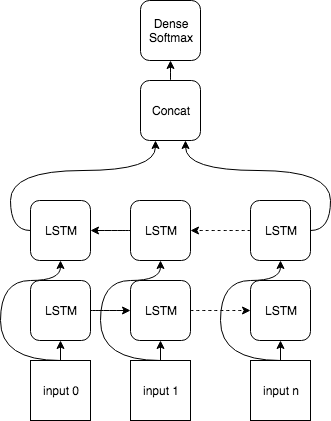
\includegraphics[width=0.5\linewidth]{Baseline}
%	\end{center}
  
   % \caption{\footnotesize{Чёрный квадрат}}
%\label{fig:square}
%\end{figure}

%На картинку тоже можно ссылаться: \cref{fig:square}

%\section{Теорема Сосницкого}
%Следующая теорема даёт ответы на все ваши вопросы.

%\begin{theorem}[Теорема Сосницкого]\label{th:sosnitsky}
%Lorem ipsum dolor sit amet, consectetur adipiscing elit.
%\end{theorem}

%Для доказательства теоремы понадобится следующая лемма:

%\begin{lemma}\label{le:sosnyakovsky}
%Если в кране нет воды, значит выпили жиды.
%\end{lemma}
%\begin{proof}
%Если в кране есть вода, значит жид нассал туда.

%\end{proof}

%\begin{enumerate}
%\item Пер.
%\item Пер.
%\item Пер.
%\end{enumerate}

%\begin{corollary}\label{cor:erofeev}
%О, тщета! О, эфемерность! 
%\end{corollary}
%\begin{proof}
%О, самое бессильное и позорное время в жизни моего народа – время от рассвета до открытия магазинов! Сколько лишних седин оно вплело во всех нас, в бездомных и тоскующих шатенов!
%\end{proof}

%\chapter{Как рисовать всякие красивости}

%\section{Система нумерованных уравнений}
%\begin{align}
%\label{eq:adin} \frac{dq}{dt} &= \frac{dH}{dp} \\
%\label{eq:dva} \frac{dp}{dt} &= -\frac{dH}{dq}
%\end{align}
%А всё для того, чтобы сослаться раз (\ref{eq:adin}), сослаться два (\ref{eq:dva})
%\begin{table}[H]\label{table:rokk_ebol}
%\begin{small}
%\begin{center}
%\begin{tabular}{|c|c|c|c|}
%\hline
%Р & О & К & К\\
%\hline
%Е & Б & О & Л\\
%\hline
%М & У & П & Ю\\
%\hline
%О & В & И & Ч\\
%\hline
%Н & И & R & Е\\
%\hline
%Т &   &   & Й\\
% абсв & & & \\
%\hline
%\end{tabular}
%\end{center}
%\end{small}
%\caption{ Sample text.}

%\end{table}

%Что бы вы думали можно сделать с \cref{table:rokk_ebol}

%\section{Дерево}
%Хер знает зачем, но вдруг пригодится.

%\begin{figure}[H]
%\Tree[.(start) [.РОКК  [.р [.о [.к ] ] ]
   %                     [.к [.е [.б ] ]
      %                          [.о [.л ] ] ] ]
         %      [.ЕБОЛ  [.Lorem [.Ipsum [.Dolor ] ] ]
            %            [.Set [.Amet [.fgs ] ]
               %                 [.fds [.foobar ] ] ] ]
%               [.МУПЮ ]
   %            [.ОВИЧ [.раз [.раз [.раз ] ] ]
      %                     [.это [.хард [.басс ] ]
         %                              [.саня [.колбасёр ] ] ] ] ]
%    \caption{\footnotesize{Смотри как умею}}
%\label{fig:tree}
%\end{figure}
%Опа \cref{fig:tree}. 
\newpage
\chapter*{Заключение}
\addcontentsline{toc}{chapter}{Заключение}
\section*{Итоги работы}
\addcontentsline{toc}{section}{Итоги работы}
\section*{Дальнейшие исследования}
\addcontentsline{toc}{section}{Дальнейшие исследования}


\newpage
\addcontentsline{toc}{chapter}{Список использованных источников}
\bibliography{references}

\end{normalsize}

\end{document}
